\documentclass[11pt]{article}
\usepackage[utf8]{inputenc}
\usepackage[T1]{fontenc}
\usepackage[spanish,es-noshorthands]{babel}
\usepackage[margin=2.5cm]{geometry}
\usepackage{amsmath,amssymb}
\usepackage{graphicx}
\usepackage{booktabs}
\usepackage{xcolor}
\usepackage[colorlinks=true,linkcolor=blue,citecolor=blue]{hyperref}
\usepackage{caption}
\usepackage{parskip}
\usepackage[expansion=false]{microtype}
\sloppy

\title{\textbf{¿Por qué falló la estimación de $\beta$ a INL alto?}\\
\large Re-estudio de \texttt{beta\_pred\_formula()} en el rango INL $\in[10^{-3},\,2\times10^{-1}]$}
\author{Walter Quiñonez}
\date{Reporte generado con Claude Code \textperiodcentered\ 12 de septiembre de 2026}

\begin{document}
\maketitle

\begin{quote}\itshape
Al correr el experimento de \texttt{prompt.txt} (a\_pot=5.85, INL$\approx$2$\times10^{-1}$,
batch\_number=1), la búsqueda automática de $\beta$ eligió $\beta=1389$ mientras la fórmula
analítica predecía 86.8 -- un factor 16$\times$, el máximo que permite la red de seguridad de
expansión. Se pidió re-estudiar la estimación de $\beta$ para el rango de INL 2$\times10^{-1}$
a $10^{-3}$. \textbf{Conclusión principal}: la fórmula NO está rota en ese rango --evaluada
contra las 30 combinaciones de fuerza bruta disponibles hoy da mediana de error 0.94$\times$ y
peor caso 1.26$\times$, y reajustarla con más datos no mejora nada--. La causa real es otra:
todo el ground truth (y por lo tanto la fórmula) fue generado con \texttt{batch\_number=32},
una variable que ni la fórmula ni la búsqueda automática modelan. Un chequeo empírico barato
confirma que a \texttt{batch\_number=1} el $\beta$ óptimo real es varias veces más grande que a
\texttt{batch\_number=32}, para el mismo INL.
\end{quote}

\tableofcontents

\section{Contexto: qué pasó y qué se pidió}

Corriendo \texttt{Crossbar\_train\_experimento\_beta\_por\_capa.py} con los parámetros de
\texttt{prompt.txt} (a\_pot=a\_dep=5.85, pulsos=50, concavidad pos/neg, \texttt{batch\_number=1},
\texttt{optimize\_beta=True}), \texttt{search\_best\_beta\_mejorado} centró su grilla en
$\beta_{\text{pred}}=86.8$ (fórmula analítica de \texttt{formula\_beta\_optimo\_propuesta/}),
pero el óptimo empírico de la búsqueda se fue corriendo hacia arriba en cada expansión hasta
$\beta=1389$ (factor $16\times=4\times4\times$ el margen, el techo con
\texttt{max\_expansiones=2}), sin encontrar un pico real. Esto se interpretó como que ``la
estimación estaba fallando'' para este INL, y se pidió re-estudiarla incluyendo el rango
INL $\in[10^{-3},\,2\times10^{-1}]$.

\section{Primera hipótesis: ¿la fórmula falla en este rango de INL?}

El ground truth de fuerza bruta en \texttt{data\_beta\_grid\_search\_SP/} ya cubre justo este
rango y más: 10 valores de INL nominal (2$\times10^{-1}$ hasta 4.82$\times10^{-6}$) $\times$ 3
cantidades de pulsos = 30 combinaciones, cada una con 20 series $\times$ 5 folds $\times$ 100
épocas reales. La fórmula en producción (\texttt{beta\_pred\_formula}, coeficientes ajustados
sobre 18 de esas 30 curvas) se re-evaluó -sin volver a entrenar nada, el Monte Carlo de
$\sigma_W$/paso\_medio tarda milisegundos- restringida a las 15 combinaciones con INL en
$[10^{-3},\,2\times10^{-1}]$, y se comparó contra dos reajustes alternativos validados por
leave-one-out cross-validation (para no premiar sobreajuste):

\begin{table}[htbp]
\centering
\begin{tabular}{@{}lrrr@{}}
\toprule
Modelo & mediana(ratio) & rango(ratio) & RMSE(log ratio) \\
\midrule
\textbf{v2 producción} (sin reajustar) & \textbf{0.940} & \textbf{[0.733, 1.264]} & \textbf{0.172} \\
Reajuste con 30 combos (LOOCV) & 0.963 & [0.729, 1.500] & 0.194 \\
Reajuste solo del rango pedido (LOOCV) & 0.971 & [0.724, 1.473] & 0.204 \\
\bottomrule
\end{tabular}
\caption{Error de predicción ($\beta_{\text{pred}}/\beta_{\text{óptimo real}}$), los 3 modelos
evaluados SOLO en las 15 combinaciones INL $\in[10^{-3}, 2\times10^{-1}]$. Script:
\texttt{reestimar\_formula\_beta\_optimo.py}.}
\end{table}

La fórmula que ya está en producción es, de las tres, la que \textbf{mejor generaliza} en este
rango -ni agregar las 12 combinaciones nuevas ni especializar el ajuste al rango mejora el
error-. Ver Figura~\ref{fig:comparacion_modelos}. Esto descarta la hipótesis de que la fórmula
esté ``rota'' para INL alto: para $\beta_{\text{pred}}=86.8$ contra el óptimo real de $\beta=100$
(INL=2$\times10^{-1}$, p=50, \texttt{batch\_number=32}) el ratio es 0.868, dentro de lo esperado.

\begin{figure}[htbp]
\centering
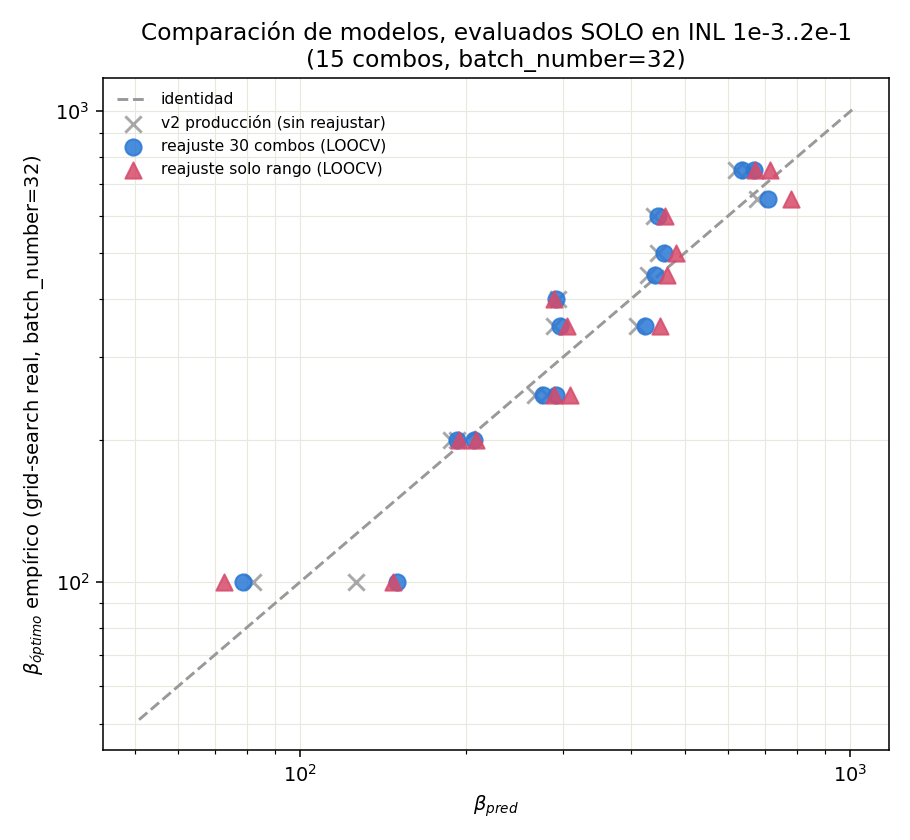
\includegraphics[width=0.72\textwidth]{comparacion_modelos_rango.png}
\caption{$\beta_{\text{pred}}$ de los 3 modelos vs. $\beta_{\text{óptimo}}$ real (fuerza bruta,
batch\_number=32), restringido a INL $\in[10^{-3},2\times10^{-1}]$ (15 combos). Los tres caen
casi sobre la identidad.}
\label{fig:comparacion_modelos}
\end{figure}

\section{La causa real: \texttt{batch\_number}, una variable no modelada}

Si la fórmula predice bien para \texttt{batch\_number=32} (el único régimen con ground truth),
¿por qué la búsqueda automática -corriendo con \texttt{batch\_number=1}, como pedía
\texttt{prompt.txt}- se fue tan lejos de esa predicción? Hipótesis: \texttt{batch\_number}
determina cuántas actualizaciones de pulso ocurren por época (\texttt{batch\_number} pasos, cada
uno sobre una fracción del dataset), y el $\beta$ óptimo depende fuertemente de cuántas
actualizaciones totales va a recibir el crossbar durante el entrenamiento -algo que ni la
fórmula (funciones solo de la curva P/D) ni el ground truth (siempre corrido a
\texttt{batch\_number=32}) contemplan.

\subsection{Chequeo empírico}

Para confirmarlo sin correr una fuerza bruta completa, se entrenó el mismo caso
(INL=2$\times10^{-1}$, p=50, a\_pot=5.85) con \texttt{batch\_number=1}, 100 épocas, 5 folds,
pero con $\beta$ \textbf{fijo} (sin búsqueda) en 3 valores nuevos (50, 100, 300), más el
$\beta=1389$ ya entrenado por la búsqueda automática (\texttt{MLP\_test\_SP/}):

\begin{table}[htbp]
\centering
\begin{tabular}{@{}rr@{}}
\toprule
$\beta$ (fijo) & accuracy final (media, 5 folds) \\
\midrule
50 & 0.6313 \\
100 & 0.6356 \\
300 & 0.6505 \\
1389 & 0.7004 \\
\bottomrule
\end{tabular}
\caption{\texttt{batch\_number=1}, 100 épocas, 5 folds, INL=2$\times10^{-1}$, p=50. Accuracy
sigue subiendo monótonamente hasta $\beta=1389$ -no se llegó todavía al pico real-.}
\end{table}

Confirmado: a \texttt{batch\_number=1} un $\beta$ mucho más grande de verdad da mejor accuracy
-no fue un artefacto de la búsqueda corta (8 épocas) ni de la expansión automática-. La
Figura~\ref{fig:bn1_vs_bn32} contrasta esta curva con el ground truth completo a
\texttt{batch\_number=32} para el mismo INL: a bn=32 el óptimo es un pico agudo en
$\beta\approx100$ (accuracy $\approx0.85$) que colapsa rápido para $\beta$ mayores; a bn=1 la
curva sube lento y sigue subiendo más allá de $\beta=1389$, sin haber encontrado su pico.

\begin{figure}[htbp]
\centering
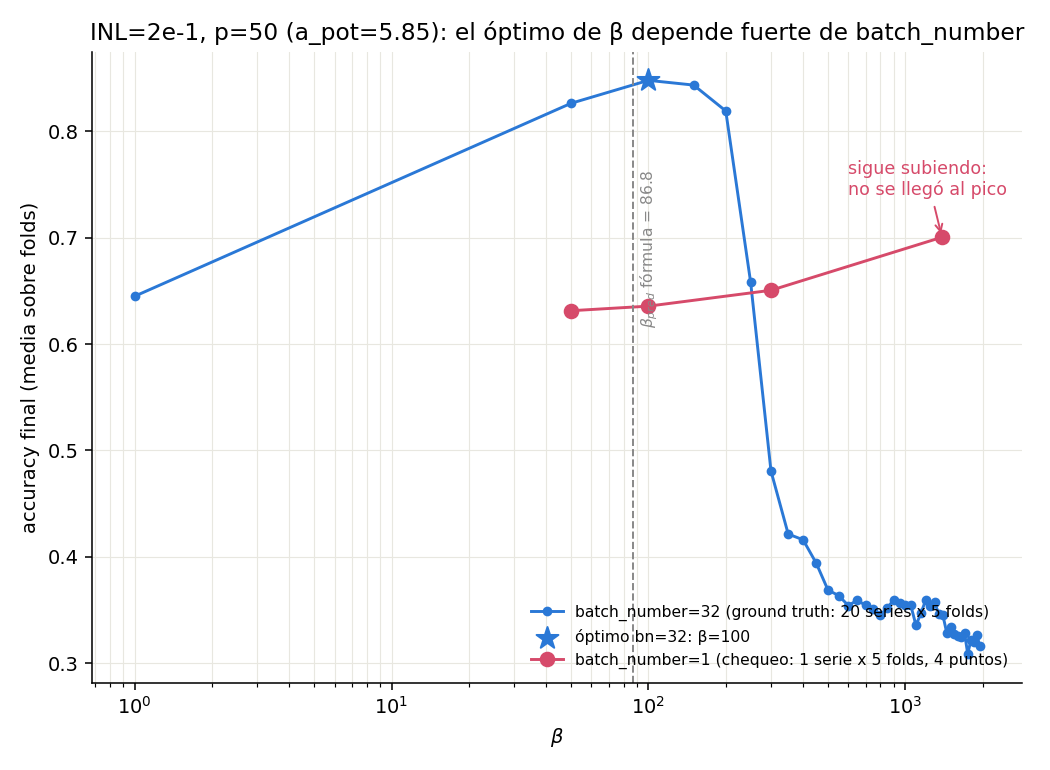
\includegraphics[width=0.85\textwidth]{chequeo_batch_number/comparacion_bn1_vs_bn32.png}
\caption{Accuracy vs. $\beta$ para el mismo INL/pulsos, a \texttt{batch\_number=32} (ground
truth completo) vs. \texttt{batch\_number=1} (chequeo barato, 4 puntos). El óptimo se desplaza
más de un orden de magnitud.}
\label{fig:bn1_vs_bn32}
\end{figure}

\section{Recomendaciones}

\begin{enumerate}
\item \textbf{No hace falta re-derivar \texttt{beta\_pred\_formula}}: ya generaliza bien
($\pm$26-30\%) en todo el rango INL $[10^{-3}, 2\times10^{-1}]$ para el régimen en el que hay
ground truth (\texttt{batch\_number=32}). Reajustarla con más datos no ayuda (Sección 2).
\item \textbf{\texttt{batch\_number} lejos de 32 invalida el centro de la grilla}: cuando se
corra con un \texttt{batch\_number} muy distinto al del ground truth (como
\texttt{batch\_number=1} en \texttt{prompt.txt}), tratar la predicción de la fórmula solo como
un punto de partida, no como un resultado confiable -la red de seguridad de
\texttt{search\_best\_beta\_mejorado} (\texttt{margen}, \texttt{max\_expansiones}) es la que
sostiene la precisión en ese caso, y puede necesitar más margen del default (el chequeo de este
informe ni siquiera llegó al pico real con $16\times$ de margen).
\item \textbf{Corto plazo, sin código nuevo}: si se sabe de antemano que \texttt{batch\_number}
será chico, llamar a \texttt{search\_best\_beta\_mejorado} con \texttt{margen} y/o
\texttt{max\_expansiones} más generosos (ya son parámetros expuestos, no hace falta tocar
código) para no cortar la expansión antes de encontrar el pico real.
\item \textbf{Mediano plazo}: generar ground truth de fuerza bruta a \texttt{batch\_number}
chico (an{\'a}logo a \texttt{data\_beta\_grid\_search\_SP/} pero variando \texttt{batch\_number}
en vez de INL) permitiría ajustar una fórmula que incluya el número total de actualizaciones
(\texttt{epochs}$\times$\texttt{batch\_number}) como variable explícita -queda fuera del alcance
de este informe por el costo de cómputo (cada combo de fuerza bruta completo tarda horas).
\end{enumerate}

\section{Limitaciones}

\begin{itemize}
\item El chequeo de \texttt{batch\_number=1} usa 1 serie y 4 valores de $\beta$ (no 20 series
y 40 valores como el ground truth completo) -suficiente para confirmar la dirección y magnitud
del efecto, no para fijar un $\beta_{\text{óptimo}}$ preciso a \texttt{batch\_number=1}: la
curva de la Figura~\ref{fig:bn1_vs_bn32} ni siquiera encontró su pico.
\item Solo se probó un combo (INL=2$\times10^{-1}$, p=50); no se verificó si la magnitud del
efecto de \texttt{batch\_number} es la misma en otros INL del rango pedido.
\item El re-ajuste de la fórmula (Sección 2) sigue sin optimizar $\beta$ distintos por capa, ni
contempla otras arquitecturas o ratios Gmax/Gmin (misma limitación que las versiones
anteriores).
\end{itemize}

Scripts y datos: \texttt{reestimar\_formula\_beta\_optimo.py} (re-ajuste y LOOCV, no entrena
nada) y \texttt{chequeo\_batch\_number/} (los 3 entrenamientos reales a beta fijo, sus
\texttt{.npz}/\texttt{.json} y el script de la Figura~\ref{fig:bn1_vs_bn32}), ambos en esta
misma carpeta.

\end{document}
